\subsection{Time Series Analysis}

\subsubsection{Trend Model}

\begin{definition} \hlt{Linear Trend Model}\\
Dependent variable changes at a constant rate with them.
\begin{equation}
y_t = b_0 + b_1 t + \epsilon_t, \ \ \ t \in {1, \ldots, T} \nonumber
\end{equation}
Ordinary Least Squares (OLS) is used to estimate coefficient, to get $\hat{Y}_t = \hat{B}_0 + \hat{B}_1 (t)$\\
Trend models may use Durbin-Watson test for serial correlation.
\end{definition}

\begin{definition} \hlt{Log-Linear Trend Models}\\
Used in cases where there is exponential growth.
\begin{equation}
\ln (y_t) = b_0 + b_1 t + \epsilon_t, \ \ \ t \in {1, \ldots, T} \nonumber
\end{equation}
\end{definition}

\begin{figure}[H]
\centering
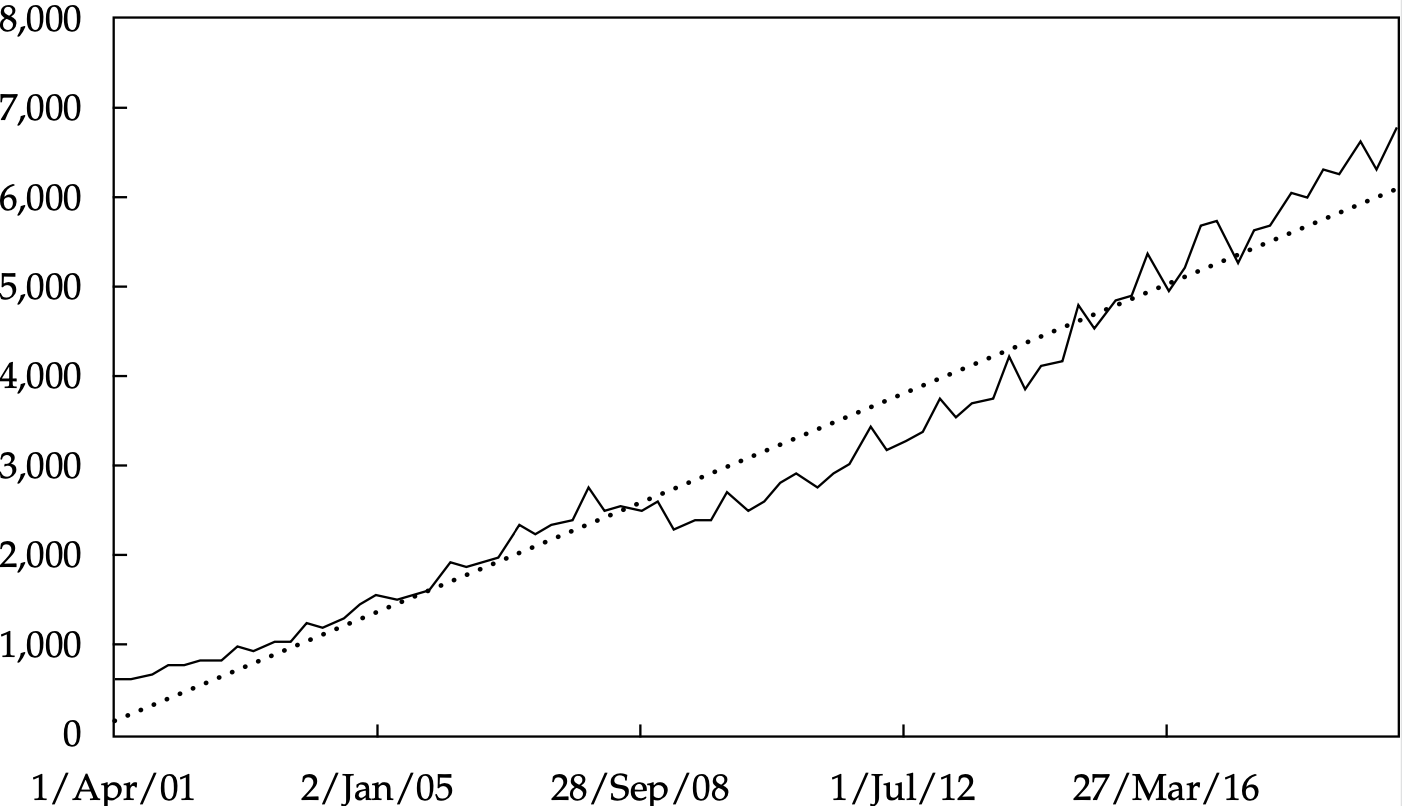
\includegraphics[scale=0.27]{/quant/lintrend}
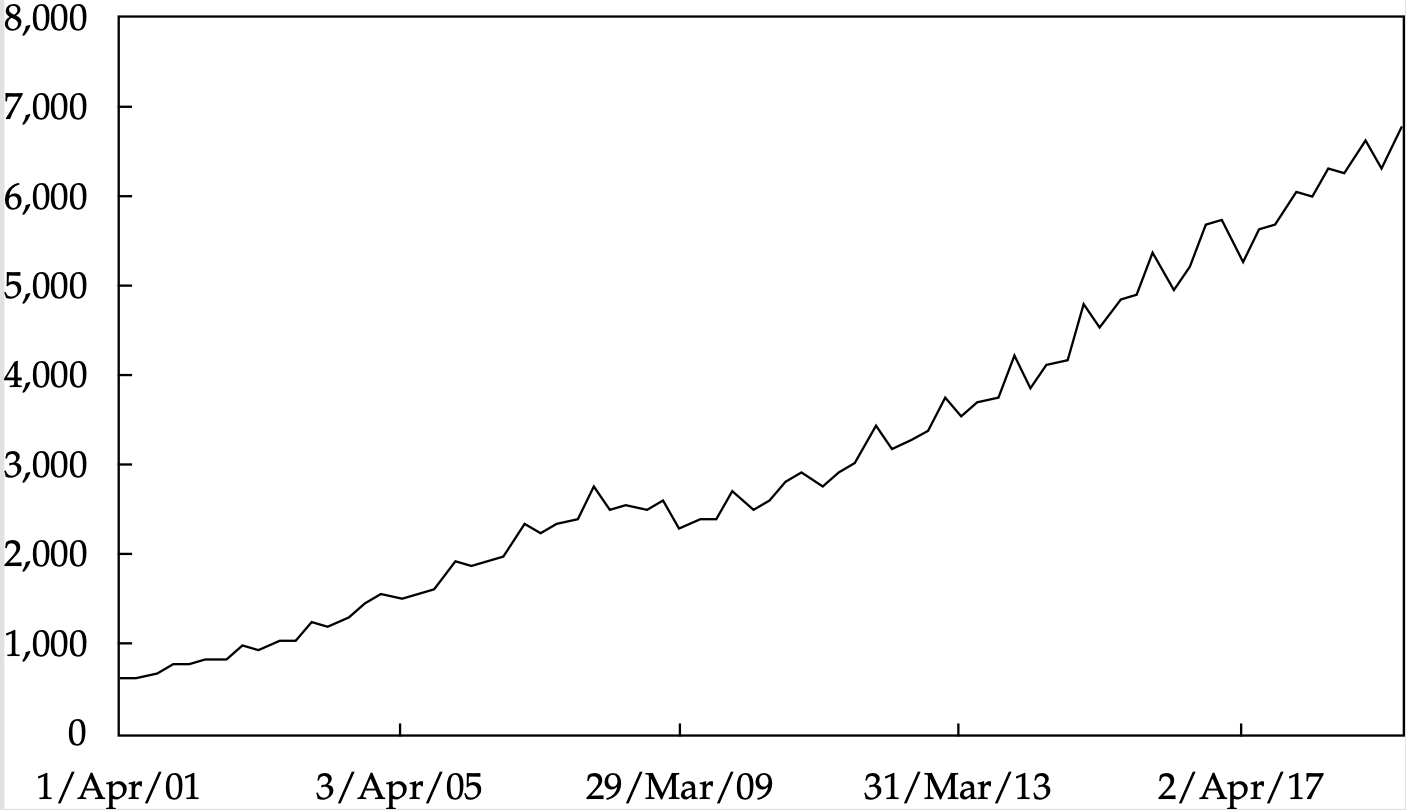
\includegraphics[scale=0.27]{/quant/exptrend}
\caption{Linear trend, exponential trend}
\end{figure}

\subsubsection{AR Models}

\begin{definition} \hlt{Autoregressive (AR) Model of Order $p$}\\
Dependent variable is regressed against one or more lagged values of itself. For a model of order $p$, AR($p$),
\begin{equation}
x_t = b_0 + \sum\limits_{i=1}^p b_i x_{t-p} + \epsilon_t \nonumber
\end{equation}
\end{definition}

\begin{definition} \hlt{Covariance Stationary}\\
Statistical inference based on OLS estimates for AR($p$) model is invalid unless time series is covariance stationary:
\begin{enumerate}[label=\roman*.]
\setlength{\itemsep}{0pt}
\item Constant and finite expected value (expected value is constant over time; mean-reverting)
\item Constant and finite variance (volatility around its mean does not change over time)
\item Constant and finite covariance between values at any given lag
\end{enumerate}
\end{definition}

\begin{remark} \hlt{Test of Autocorrelation}
\begin{enumerate}[label=\roman*.]
\setlength{\itemsep}{0pt}
\item Compute the AR($p$) model using linear regression
\item Calculate the autocorrelation of the model residuals.\\
Note, the $k$-th order estimated autocorrelation $\hat{\rho}_k$ and autocorrelations of error term $\rho_{\epsilon, k}$ are as follows
\begin{align}
\hat{\rho}_k = \frac{\sum\limits_{t=k+1}^T [(x_t - \overline{x}) (x_{t-k} - \overline{x})]}{\sum\limits_{t=1}^T (x_t - \overline{x})^2}, \ \ \ \ \rho_{\epsilon, k} = \frac{E(\epsilon_t \epsilon_{t-k})}{\sigma_{\epsilon}^2} \nonumber
\end{align}
\item Test if the residual correlations are significantly from zero.\\
If model is correctly specified, none of the autocorrelations will be statistically significant.\\
To test for significant,$H_0: \rho_{\epsilon, k} = 0$ and $H_a: \rho_{\epsilon, k} \neq 0$.  $t$-statistic with $df = T-2$ is
\begin{equation}
t = \frac{\rho_{\epsilon, k}}{1/\sqrt{T}} \nonumber
\end{equation}
Note the standard error of residual correlation is $1/\sqrt{T}$.
\end{enumerate}
\end{remark}

\begin{remark} \hlt{Mean Reversion}\\
Time series exhibits tendency to move towards its mean.\\
For AR($1$), mean reverting is when $x_t = b_0 + b_1 x_t$, hence mean reverting level is $x_t = \frac{b_0}{1-b_1}$.\\
All covariance stationary time series have a finite mean-reverting level.
\end{remark}

\begin{remark} \hlt{Types of Forecasts}
\begin{enumerate}[label=\roman*.]
\setlength{\itemsep}{0pt}
\item In-Sample Forecasts: $\hat{Y}$ made within the range of data used to estimate the model.
\item Out-of-Sample Forecasts: made outside of the sample period, provides test of whether model has predictive power in real world.
\end{enumerate}
\end{remark}

\begin{remark} \hlt{Root Mean Squared Error (RMSE)}\\
RMSE is used to compare accuracy of AR($p$) models for out-of-sample values.
\begin{equation}
RMSE = \sqrt{\sum\limits_{i=1}^n \frac{(\hat{Y}_i - Y_i)^2}{n}} \nonumber
\end{equation}
where $\hat{Y}_i$ are predicted values, $Y_i$ are actual values, $n$ is number of observations.\\
Model with lowest RMSE for in-sample data may not be model with lowest RMSE for out-of-sample data.\\
Model with lower RMSE for out-of-sample data will have lower forecast error and better predictive power.
\end{remark}

\begin{definition} \hlt{Random Walk}\\
Time series in which the value of the series in one period is the value of the series in the previous period plus an unpredictable random error.
\begin{align}
x_t &= x_{t-1} + \epsilon_t \nonumber \\
E[\epsilon_t] &= 0, E[\epsilon_t^2] = \sigma^2 \nonumber \\
\text{Cov}[\epsilon_t, \epsilon_s] &= E[\epsilon_t \epsilon_s] = 0 \ \ \text{if} \ \ i \neq j \nonumber
\end{align}
Expected value of error is zero, variance of error is constant, there is no serial correlation in error.
\end{definition}

\begin{definition} \hlt{Random Walk with Drift}\\
Time series expected to increase or decrease by a constant amount each period.
\begin{equation}
x_t = b_0 + b_1 x_{t-1} + \epsilon_t \nonumber
\end{equation}
\end{definition}

\begin{remark} \hlt{Properties of Random Walk}\\
Random walk has an undefined mean-reverting level ($\frac{b_0}{1-b_1} = \frac{b_0}{0}$), hence is not covariance stationary.\\
All random walks have a unit root $b_1 = 1$, hence least squares regression cannot be used.
\end{remark}

\begin{definition} \hlt{First Difference}\\
Subtracts value of the time series in the first prior period from the current value of the time series.
\begin{equation}
\Delta x_t = x_t - x_{t-1} \nonumber
\end{equation}
\end{definition}

\begin{remark} \hlt{Dickey-Fuller Unit Root Test}\\
Given an AR($1$) model $x_t = b_1 x_{t-1} + \epsilon_t$, take the first difference to get $\Delta x_t = (b_1 - 1)x_{t-1} + \epsilon_t$.\\
Let $g_1 = b_1 -1 $. If there is a unit root in the model, then $g_1 = 0$.\\
Hypothesis test is then $H_0: g_1 = 0$ (has unit root, non-stationary), and $H_a: g_1 < 0$ (no unit root, stationary)\\
$t$-statistic is computed in a conventional manner for $\hat{g}_1$, but a revised set of values are used for the test.
\end{remark}

\begin{remark} \hlt{Seasonality}\\
Pattern that tends to repeat form year to year.\\
To adjust for seasonality in an AR($p$) model, add additional lag, i.e., $x_t = b_0 + b_1 x_{t-1} + b_2 x_{t-4} + \epsilon_t$
\end{remark}

\subsubsection{ARMA, ARCH Models}

\begin{definition} \hlt{Moving Average (MA) Models}\\
The MA($q$) model is as follows:
\begin{align}
x_t = \mu + \sum\limits_{i=1}^q \theta_i \epsilon_{t-i} + \epsilon_t, \ \ \ E[\epsilon_t] = 0, E[\epsilon_t^2] = \sigma^2, \text{Cov}[\epsilon_t, \epsilon_s] = E[\epsilon_t \epsilon_s] = 0 \ \ \text{for} \ \ t \neq s \nonumber
\end{align}
where $\mu$ is mean of the series, $\theta$ are coefficients of the series
\end{definition}

\begin{definition} \hlt{Autoregressive Moving Average (ARMA) Model}\\
Combines both autoregressive lags of dependent variable and moving-average errors. ARMA($p,q$) is as follows:
\begin{equation}
x_t = b_0 + \sum\limits_{i=1}^p b_i x_{t-i} + \mu + \sum\limits_{i=1}^q \theta_i \epsilon_{t-i} + \epsilon_t, \ \ \ E[\epsilon_t] = 0, E[\epsilon_t^2] = \sigma^2, \text{Cov}[\epsilon_t, \epsilon_s] = E[\epsilon_t \epsilon_s] = 0 \ \ \text{for} \ \ t \neq s \nonumber
\end{equation}
Note that parameters in ARMA models can be very unstable to slight perturbations.\\
Choosing the right $p,q$ values is more of an art than a science, as criteria for choosing is far from perfect.\\
Even after a model is selected, the model may not forecast well.
\end{definition}

\begin{definition} \hlt{Autoregressive Conditional Heteroskedasticity (ARCH) Model}\\
Used to test for autoregressive conditional heteroskedasticity. The time series variance of residuals in on e period is dependent on variance of residuals in preceding periods. An ARCH($q$) mode is as follows
\begin{equation}
\epsilon_t \sim N \left( 0, a_0 + \sum\limits_{i=1}^q a_i \epsilon_{t-1}^2 \right), \ \ \ \epsilon_t^2 = a_0 + \sum\limits_{i=1}^q a_i \epsilon_{t-1}^2 \nonumber
\end{equation}
Using $t$-statistics, if $a_i$ is statistically significant from zero, then series is ARCH($q$).
\end{definition}

\subsubsection{Regression on Multiple Timeseries}

\begin{remark} \hlt{Multiple Timeseries Regression}\\
To regress a time series $y_t$ on another time series $x_t$, i.e., $y_t = b_0 + b_1 x_t + \epsilon_t$.\\
As there are two different time series $x_t$ and $y_t$, either of both can be subject to non-stationarity.\\
First estimate the regression $y_t = b_0 + b_1 x_t + \epsilon_t$, then to run separate Dickey-Fuller tests with possible results:
\begin{enumerate}[label=\roman*.]
\setlength{\itemsep}{0pt}
\item Neither have unit root, i.e., both time series are covariance stationary.
\item Only dependent variable time series is covariance stationary, i.e, $H_0$ for dependent variable not rejected.
\item Only independent variable time series is covariance stationary, i.e, $H_0$ for independent variable not rejected.
\item Neither is covariance stationary, and both time series are not co-integrated.
\item Neither is covariance stationary, and both time series are co-integrated.
\end{enumerate}
For scenario $1$, linear regression may be used, and coefficients should be statistically reliable.\\
For scenario $2, 3$, linear regression may not be used, as coefficients will not be statistically reliable.\\
For scenario $4, 5$, whether linear regression can be used depends on whether two time series are co-integrated.
\end{remark}

\begin{definition} \hlt{Co-Integration of Time Series}\\
Two time series are economically linked, or follow the same trend, and relationship is not expected to change.\\
If two time series are co-integrated, the error term from regressing on eon the other is covariance stationary.
\begin{enumerate}[label=\roman*.]
\setlength{\itemsep}{0pt}
\item Estimate regression $y_t = b_0 + b_1 x_t + \epsilon_t$.
\item Test if $\epsilon_t$ has unit root with Dickey-Fuller, but use critical values by Engle and Granger (DF-EG test).
\item If test rejects $H_0$, then $\epsilon_t$ is covariance stationary, and both are co-integrated.
\end{enumerate}
\end{definition}

\begin{definition} \hlt{Steps for Time-Series Forecasting}
\begin{enumerate}[label=\roman*.]
\setlength{\itemsep}{0pt}
\item Understand investment problem, casual relationships of variables
\item Plot time series for indications of seasonality, structural shifts, linear or exponential trend.
\item If no seasonality or structural shifts, use a trend model.
\begin{enumerate}[label=\arabic*.]
\setlength{\itemsep}{0pt}
\item If data plot is a straight line, use a linear trend model
\item If data plot is a curve, use a log-linear trend model
\end{enumerate}
\item Run trend analysis, compute the residuals, test for serial correlation using Durbin-Watson test
\begin{enumerate}[label=\arabic*.]
\setlength{\itemsep}{0pt}
\item If no serial correlation, the trend model can be used.
\item If serial correlation is detected, use a more complex model
\end{enumerate}
\item If data has serial correlation, reexamine the data for stationarity before running AR model. If it is not stationary, treat the data for use in an AR model as follows:
\begin{enumerate}[label=\arabic*.]
\setlength{\itemsep}{0pt}
\item If data has linear trend, first-difference the data
\item If data has exponential trend, first-difference the natural log of the data
\item If there is structural shift in the data, run two separate models
\item If data has seasonal component, incorporate seasonality into the AR model
\end{enumerate}
\item After first-differencing, if series is covariance stationary, run AR($1$), test for serial correlation \& seasonality.
\begin{enumerate}[label=\arabic*.]
\setlength{\itemsep}{0pt}
\item If there is no remaining serial correlation, model may be used
\item If serial correlation is detected, incorporate lagged values of the variable (possibly including one for seasonality) into the AR model until serial correlation has been removed.
\end{enumerate}
\item Test residuals with ARCH. Regress square residuals on squared lagged value of residuals and test if resulting coefficient is significantly different from zero.
\begin{enumerate}[label=\arabic*.]
\setlength{\itemsep}{0pt}
\item If coefficient is not significantly different from zero, model may be used.
\item If coefficient is significantly different from zero, ARCH is present. Use generalised least squares.
\end{enumerate}
\item Perform tests of model’s out-of-sample forecasting performance with RMSE.
\end{enumerate}
\end{definition}
